% appendix.tex

\appendix

\section{Logistic Regression}

In this section, we detail the steps and results obtained from using the Logistic Regression model during the supervised learning phase of the project. Logistic Regression served as a baseline model to provide an initial understanding of the classification problem. Despite its simplicity, it offered valuable insights into the multi-label classification task.

\subsection{Model Training}
The Logistic Regression model was trained using its default configuration. Specifically, the \texttt{lbfgs} solver was utilized with a regularization parameter \( C = 1 \). The training process aimed to identify potential overfitting or underfitting issues and establish baseline performance metrics.

        \begin{lstlisting}[caption={Train Logistic Regression model}, label={lst:logistic_regression_train}]
                # Initialize and train Logistic Regression model
                model = LogisticRegression(max_iter=1000, random_state=42)
                model.fit(X_train_tfidf, y_train_binary)
        \end{lstlisting}

The dataset was preprocessed using the TF-IDF representation of the session texts, which assigned weights to words based on their frequency and relevance within the dataset. Multi-label binary encoding was applied to the `Set\_Fingerprint` column to ensure compatibility with the model.

\subsection{Evaluation Metrics}
The Logistic Regression model was evaluated using standard classification metrics, including weighted F1-scores, precision, and recall. The evaluation metrics highlighted the strengths and weaknesses of the model in handling imbalanced classes. 

        \begin{lstlisting}[caption={Generate classification report}, label={lst:logistic_regression_eval}]
                # Generate classification report
                from sklearn.metrics import classification_report
                report = classification_report(y_test_binary, y_pred, zero_division=0)
                print(report)
        \end{lstlisting}

The confusion matrix provided a breakdown of true positives, false positives, false negatives, and true negatives for each intent. Figure~\ref{fig:logistic_cm} shows the confusion matrix for the Logistic Regression model.

\begin{figure}[H]
    \centering
    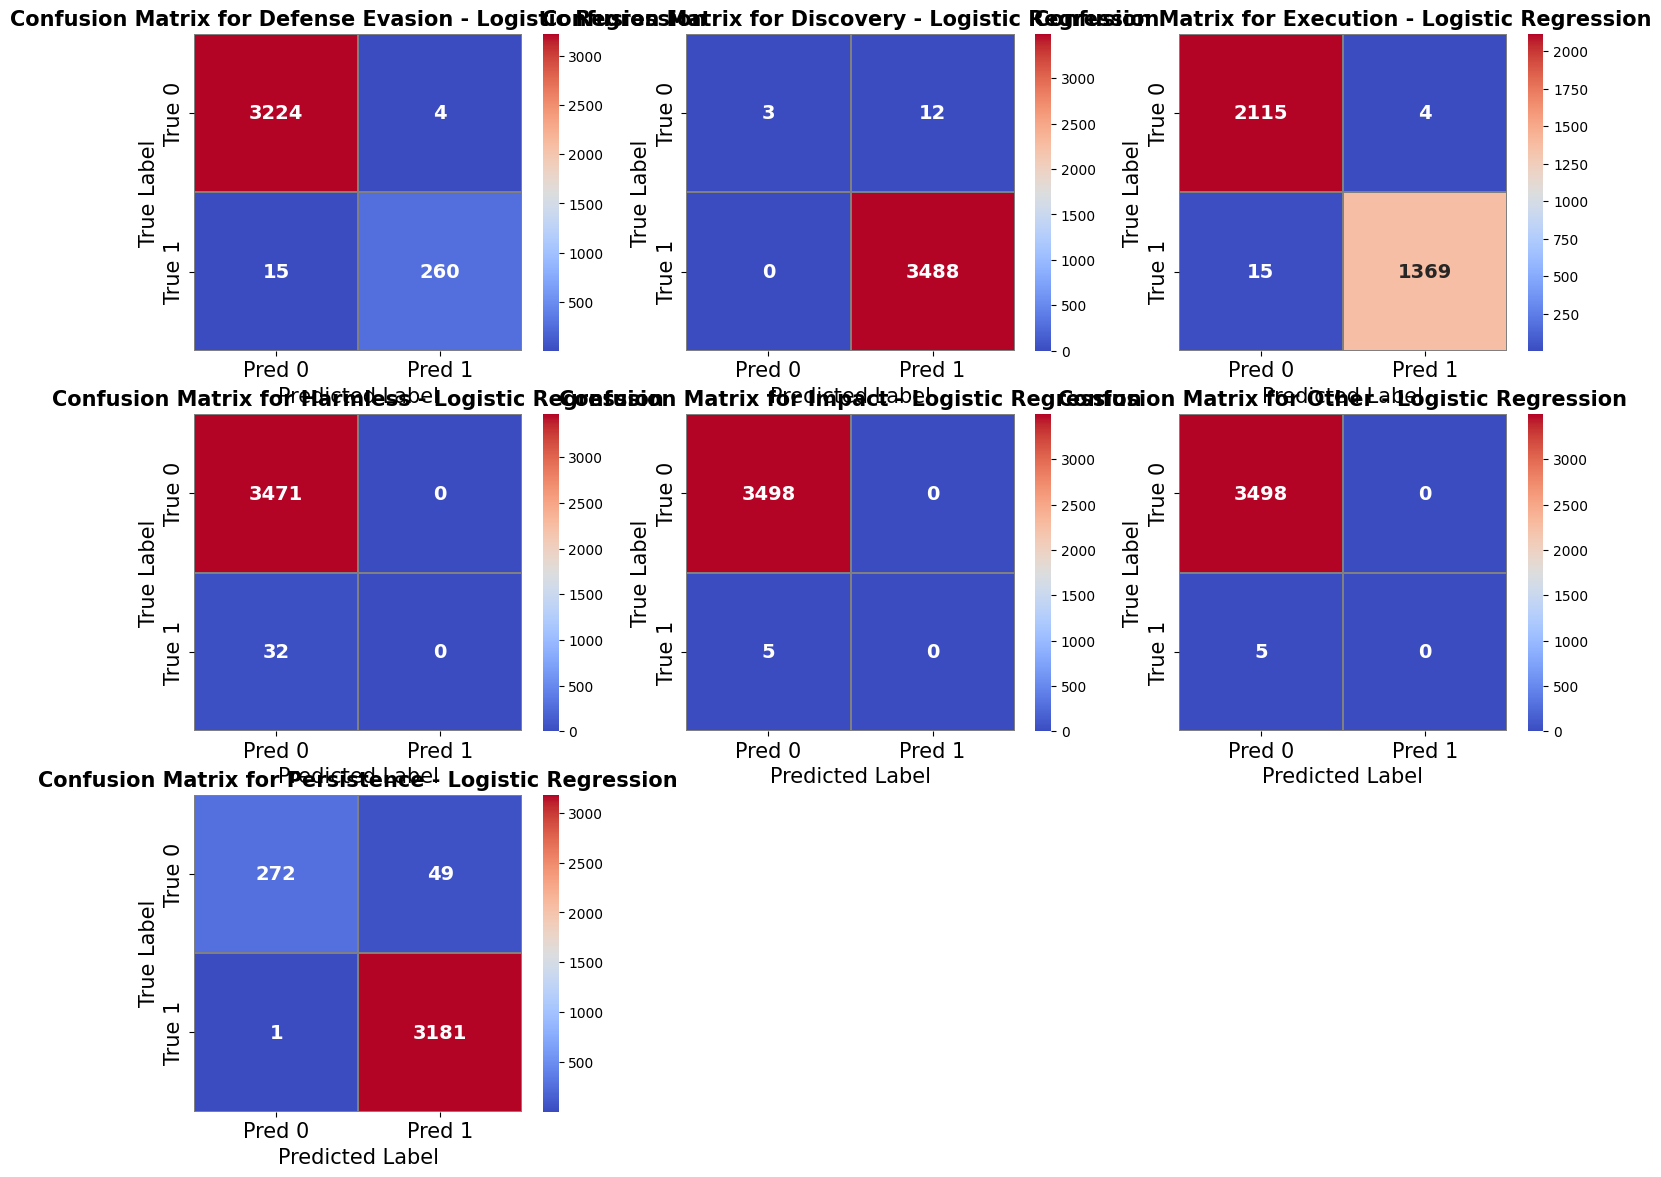
\includegraphics[width=0.8\textwidth]{../figures/plots/section2/Logistic_Regression_base_evaluation.png}
    \caption{Confusion Matrix for Logistic Regression Model.}
    \label{fig:logistic_cm}
\end{figure}

\subsection{Hyperparameter Tuning}
Grid search was performed to optimize the Logistic Regression model's hyperparameters. The search focused on varying the regularization parameter \( C \) over a range of values \([0.1, 1, 10, 100]\) to identify the configuration that maximized weighted F1-scores.

            \begin{lstlisting}[caption={Parameter grid for Logistic Regression}, label={lst:logistic_param_grid}]
                # Define parameter grid for Logistic Regression
                param_grid = {'C': [0.1, 1, 10, 100]}
                grid_search = GridSearchCV(LogisticRegression(max_iter=1000, random_state=42), param_grid, cv=5)
                grid_search.fit(X_train_tfidf, y_train_binary)
            \end{lstlisting}

The optimized model exhibited improved performance compared to the baseline, particularly for intents with smaller sample sizes. Figure~\ref{fig:logistic_tuning} illustrates the weighted F1-scores for different values of \( C \).

\begin{figure}[H]
    \centering
    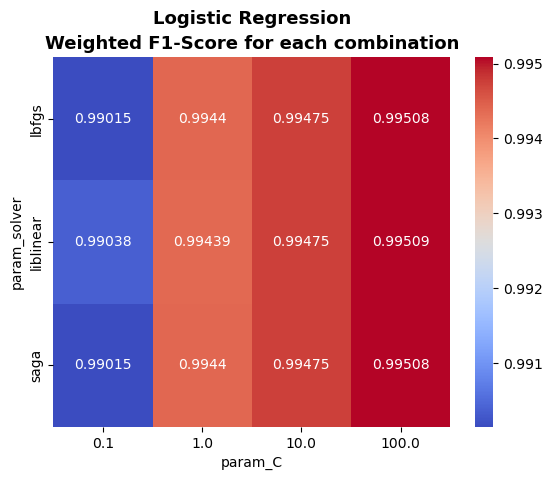
\includegraphics[width=0.8\textwidth]{../figures/plots/section2/weighted_f1_score_for_each_combination_of_parameters_logistic_regression.png}
    \caption{Weighted F1-Scores for Logistic Regression Hyperparameter Tuning.}
    \label{fig:logistic_tuning}
\end{figure}

\subsection{Comparative Analysis of Baseline and Optimized Models}
The optimized Logistic Regression model demonstrated a moderate improvement in precision and recall compared to the baseline. However, its overall performance remained slightly inferior to more complex models like Random Forest and SVM. The comparative analysis underscores the importance of selecting models suited to the dataset's characteristics and problem requirements.


\section{Code Snippets}

    % \subsection{Code Snippets}

        \subsection{Data Exploration and Pre-processing}
        % \textbf{{Data Exploration and Pre-processing}
        
            \vspace{0.5em}

            % Load and inspect the dataset
            \begin{lstlisting}[caption={Load and inspect the dataset}, label={lst:load-inspect-dataset}]
                # Load the dataset
                SSH_Attacks = pd.read_parquet("../data/processed/ssh_attacks_decoded.parquet")
        
                # Inspect the dataset structure
                print(SSH_Attacks.info())
        
                # Check for missing values
                print(SSH_Attacks.isnull().sum())
        
                # Check for duplicate rows
                print(SSH_Attacks.duplicated().sum())
            \end{lstlisting}
            
            \vspace{0.5em}

            % Convert timestamps and analyze frequencies
            \begin{lstlisting}[caption={Convert timestamps and analyze frequencies}, label={lst:convert-analyze-frequencies}]
                # Convert first_timestamp to datetime format
                SSH_Attacks['first_timestamp'] = pd.to_datetime(SSH_Attacks['first_timestamp'])

                # Analyze attack frequencies over time
                temporal_series = (
                    SSH_Attacks.groupby(SSH_Attacks['first_timestamp'].dt.date)
                    .size()
                    .reset_index(name='attack_count')
                )
            \end{lstlisting}
            
            \vspace{0.5em}

            % Extract and visualize class distribution
            \begin{lstlisting}[caption={Extract and visualize class distribution}, label={lst:extract-visualize-classes}]
                # Extract and count occurrences of each class
                all_classes = SSH_Attacks['Set_Fingerprint'].explode().str.strip()
                class_counts = all_classes.value_counts()

                # Plot the distribution of classes
                sns.barplot(x=class_counts.index, y=class_counts.values, palette='viridis')
            \end{lstlisting}
            
            \vspace{0.5em}

            % Generate a word cloud from session text
            \begin{lstlisting}[caption={Generate a word cloud from session text}, label={lst:generate-wordcloud}]
                # Generate a word cloud for the session text
                wordcloud = WordCloud(width=800, height=400, background_color='white').generate(' '.join(SSH_Attacks['Full session text']))
                plt.imshow(wordcloud, interpolation='bilinear')
                plt.axis('off')
                plt.show()
            \end{lstlisting}
            
            \vspace{0.5em}

            % Group attacks by fingerprint and date
            \begin{lstlisting}[caption={Group attacks by fingerprint and date}, label={lst:group-attacks}]
                # Group by Set_Fingerprint and date to count occurrences
                grouped_SSH_Attacks = (
                    SSH_Attacks.explode('Set_Fingerprint')
                    .groupby([SSH_Attacks['first_timestamp'].dt.date, 'Set_Fingerprint'])
                    .size()
                    .reset_index(name='attack_count')
                )
            \end{lstlisting}
            
            \vspace{0.5em}

            % Convert text into numerical representations
            \begin{lstlisting}[caption={Convert text into numerical representations}, label={lst:convert-text-numerical}]
                # Convert text into numerical representations using Bag of Words (BoW)
                from sklearn.feature_extraction.text import CountVectorizer
                bow_vectorizer = CountVectorizer()
                X_bow = bow_vectorizer.fit_transform(SSH_Attacks['Full session text'])

                # Convert text into numerical representations using TF-IDF
                from sklearn.feature_extraction.text import TfidfVectorizer
                tfidf_vectorizer = TfidfVectorizer()
                X_tfidf = tfidf_vectorizer.fit_transform(SSH_Attacks['Full session text'])
            \end{lstlisting}
            
            \vspace{0.5em}

        \subsection{Supervised Learning - Classification}
        % \textbf{Supervised Learning - Classification}
        
            \vspace{0.5em}

            % Load the dataset
            \begin{lstlisting}[caption={Load the dataset}, label={lst:load_dataset}]
                # Load the dataset
                SSH_Attacks = pd.read_parquet("../data/processed/ssh_attacks_decoded.parquet")
            \end{lstlisting}
            
            \vspace{0.5em}
            
            % Split the dataset into training and test sets
            \begin{lstlisting}[caption={Split the dataset into training and test sets}, label={lst:split_dataset}]
                # Split the dataset into training and test sets
                X_train, X_test, y_train, y_test = train_test_split(
                    X, y, test_size=0.3, random_state=42
                )
            \end{lstlisting}
            
            \vspace{0.5em}
            
            % Train Logistic Regression model
            \begin{lstlisting}[caption={Train Logistic Regression model}, label={lst:logistic_regression}]
                # Initialize and train Logistic Regression model
                model = LogisticRegression(max_iter=1000, random_state=42)
                model.fit(X_train_tfidf, y_train_binary)
            \end{lstlisting}
            
            \vspace{0.5em}
            
            % Train Random Forest model
            \begin{lstlisting}[caption={Train Random Forest model}, label={lst:random_forest}]
                # Initialize and train Random Forest model
                model = RandomForestClassifier(n_estimators=100, random_state=42)
                model.fit(X_train_tfidf, y_train_binary)
            \end{lstlisting}
            
            \vspace{0.5em}
            
            % Train SVM model
            \begin{lstlisting}[caption={Train SVM model}, label={lst:svm}]
                # Initialize and train SVM model
                model = SVC(kernel='linear', random_state=42)
                model.fit(X_train_tfidf, y_train_binary)
            \end{lstlisting}
            
            \vspace{0.5em}
            
            % Define parameter grid for Logistic Regression
            \begin{lstlisting}[caption={Parameter grid for Logistic Regression}, label={lst:param_grid_logistic}]
                # Define parameter grid for Logistic Regression
                param_grid = {'C': [0.1, 1, 10, 100]}
                grid_search = GridSearchCV(LogisticRegression(max_iter=1000, random_state=42), param_grid, cv=5)
                grid_search.fit(X_train_tfidf, y_train_binary)
            \end{lstlisting}
            
            \vspace{0.5em}
            
            % Define parameter grid for Random Forest
            \begin{lstlisting}[caption={Parameter grid for Random Forest}, label={lst:param_grid_rf}]
                # Define parameter grid for Random Forest
                param_grid = {'n_estimators': [50, 100, 200]}
                grid_search = GridSearchCV(RandomForestClassifier(random_state=42), param_grid, cv=5)
                grid_search.fit(X_train_tfidf, y_train_binary)
            \end{lstlisting}
            
            \vspace{0.5em}
            
            % Generate classification report
            \begin{lstlisting}[caption={Generate classification report}, label={lst:classification_report}]
                # Generate classification report
                report = classification_report(y_test_binary, y_pred, zero_division=0)
                print(report)
            \end{lstlisting}
            
            \vspace{0.5em}
            
            % Generate confusion matrix
            \begin{lstlisting}[caption={Generate confusion matrix}, label={lst:confusion_matrix}]
                # Generate confusion matrix
                cm = confusion_matrix(y_test_binary, y_pred)
                sns.heatmap(cm, annot=True, fmt='d', cmap='coolwarm')
                plt.show()
            \end{lstlisting}
            
            \vspace{0.5em}
            
            % Convert text using Bag of Words (BoW)
            \begin{lstlisting}[caption={Convert text using Bag of Words (BoW)}, label={lst:bow_conversion}]
                # Convert text into numerical representations using Bag of Words (BoW)
                bow_vectorizer = CountVectorizer()
                X_train_bow = bow_vectorizer.fit_transform(X_train)
                X_test_bow = bow_vectorizer.transform(X_test)
            \end{lstlisting}
            
            \vspace{0.5em}
            
            % Convert text using TF-IDF
            \begin{lstlisting}[caption={Convert text using TF-IDF}, label={lst:tfidf_conversion}]
                # Convert text into numerical representations using TF-IDF
                tfidf_vectorizer = TfidfVectorizer()
                X_train_tfidf = tfidf_vectorizer.fit_transform(X_train)
                X_test_tfidf = tfidf_vectorizer.transform(X_test)
            \end{lstlisting}
            
            \vspace{0.5em}

        \subsection{Unsupervised Learning - Clustering}
        % \textbf{Unsupervised Learning - Clustering}
        
            \vspace{0.5em}

            % Elbow Method for k-Means Clustering
            \begin{lstlisting}[caption={Elbow Method for k-Means Clustering}, label={lst:elbow_method}]
                # Elbow Method
                n_cluster_list = []
                inertia_list = []
                for n_clusters in range(3, 17):
                    kmeans = KMeans(n_clusters=n_clusters, n_init=10, random_state=42)
                    kmeans.fit(X)
                    inertia_list.append(kmeans.inertia_)
                    n_cluster_list.append(n_clusters)
                
                # Plot Elbow Method
                plt.figure(figsize=(5, 3.5))
                plt.plot(n_cluster_list, inertia_list, marker='o', markersize=5, color='blue')
                plt.xlabel('Number of clusters')
                plt.ylabel('k-Means clustering error')
                plt.title('Elbow Method')
                plt.show()
            \end{lstlisting}
            
            \vspace{0.5em}

            % Silhouette Analysis for k-Means Clustering
            \begin{lstlisting}[caption={Silhouette Analysis for k-Means Clustering}, label={lst:silhouette_analysis}]
                # Silhouette Analysis
                silhouette_list = []
                for n_clusters in range(3, 17):
                    kmeans = KMeans(n_clusters=n_clusters, n_init=10, random_state=42)
                    labels = kmeans.fit_predict(X)
                    silhouette_score_value = silhouette_score(X, labels)
                    silhouette_list.append(silhouette_score_value)
                
                # Plot Silhouette Analysis
                plt.figure(figsize=(5, 3.5))
                plt.plot(n_cluster_list, silhouette_list, marker='o', markersize=5, color='blue')
                plt.xlabel('Number of clusters')
                plt.ylabel('Silhouette Score')
                plt.title('Silhouette Analysis')
                plt.show()
            \end{lstlisting}
            
            \vspace{0.5em}

            % Grid Search for k-Means Clustering
            \begin{lstlisting}[caption={Grid Search for k-Means Clustering}, label={lst:grid_search_kmeans}]
                # Define parameter grid for K-Means
                param_grid_kmeans = {
                    'init': ['k-means++', 'random'],
                    'n_init': list(range(10, 21, 2)),
                    'max_iter': list(range(50, 200, 50)),
                }
                
                # Create KMeans object
                kmeans = KMeans(n_clusters=10, random_state=42)
                
                # Create GridSearchCV object
                grid_search_kmeans = GridSearchCV(kmeans, param_grid=param_grid_kmeans, cv=5)
                
                # Fit the grid search to the data
                grid_search_kmeans.fit(X)
                
                # Get the best parameters
                best_params_kmeans = grid_search_kmeans.best_params_
                print("Best parameters:", best_params_kmeans)
            \end{lstlisting}
            
            \vspace{0.5em}

            % Grid Search for Gaussian Mixture Model (GMM)
            \begin{lstlisting}[caption={Grid Search for Gaussian Mixture Model (GMM)}, label={lst:grid_search_gmm}]
                # Define parameter grid for GMM
                param_grid_gmm = {
                    'init_params': ['kmeans'],
                    'covariance_type': ['full', 'spherical'],
                    'tol': [1e-3, 1e-4, 1e-5],
                    'max_iter': list(range(50, 300, 50)),
                }
                
                # Create GaussianMixture object
                gmm = GaussianMixture(n_components=10, random_state=42)
                
                # Create GridSearchCV object
                grid_search_gmm = GridSearchCV(gmm, param_grid=param_grid_gmm, cv=5, scoring=silhouette_scorer)
                
                # Fit the grid search to the data
                grid_search_gmm.fit(X)
                
                # Get the best parameters
                best_params_gmm = grid_search_gmm.best_params_
                print("Best parameters:", best_params_gmm)
            \end{lstlisting}
            
            \vspace{0.5em}

            % t-SNE Visualization of Clusters
            \begin{lstlisting}[caption={t-SNE Visualization of Clusters}, label={lst:tsne_visualization}]
                # Apply t-SNE to reduce the number of components
                tsne = TSNE(n_components=2, random_state=42).fit_transform(X)
                df_tsne = pd.DataFrame(tsne, columns=['x1', 'x2'])
                
                # K-Means Clusters
                df_tsne['cluster_kmeans'] = kmeans_tuned.labels_
                sns.scatterplot(data=df_tsne, x='x1', y='x2', hue='cluster_kmeans', palette='viridis')
                plt.title('t-SNE Visualization of K-Means Clusters')
                plt.show()
                
                # GMM Clusters
                df_tsne['cluster_gmm'] = gmm_tuned.predict(X)
                sns.scatterplot(data=df_tsne, x='x1', y='x2', hue='cluster_gmm', palette='viridis')
                plt.title('t-SNE Visualization of GMM Clusters')
                plt.show()
            \end{lstlisting}
            
            \vspace{0.5em}

            % Feature Distribution Analysis by Cluster
            \begin{lstlisting}[caption={Feature Distribution Analysis by Cluster}, label={lst:feature_distribution}]
                # Analyze the distribution of features within each cluster
                for cluster in range(10):
                    cluster_data = df_tsne[df_tsne['cluster_kmeans'] == cluster]
                    print(f"Cluster {cluster} Feature Distribution:")
                    print(cluster_data.describe())
            \end{lstlisting}
            
            \vspace{0.5em}

            % Intent Proportions Analysis by Cluster
            \begin{lstlisting}[caption={Intent Proportions Analysis by Cluster}, label={lst:intent_proportions}]
                # Calculate the proportion of each intent within the clusters
                for cluster in range(10):
                    cluster_data = df_tsne[df_tsne['cluster_kmeans'] == cluster]
                    intent_proportions = cluster_data['intent'].value_counts(normalize=True)
                    print(f"Cluster {cluster} Intent Proportions:")
                    print(intent_proportions)
            \end{lstlisting}
            
            \vspace{0.5em}

            % Attack Categories Analysis by Cluster
            \begin{lstlisting}[caption={Attack Categories Analysis by Cluster}, label={lst:attack_categories}]
                # Analyze the most frequent attack categories within the clusters
                for cluster in range(10):
                    cluster_data = df_tsne[df_tsne['cluster_kmeans'] == cluster]
                    attack_categories = cluster_data['attack_category'].value_counts()
                    print(f"Cluster {cluster} Attack Categories:")
                    print(attack_categories)
            \end{lstlisting}
            
            \vspace{0.5em}

        \subsection{Language Model Exploration}
        % \textbf{Language Model Exploration}
        
            \vspace{0.5em}

            % Install required packages
            \begin{lstlisting}[language=bash, caption={Install required packages}, label={lst:install_packages}]
                !pip install transformers torch
            \end{lstlisting} 
            
            \vspace{0.5em}
            
            % Load dataset and print its size
            \begin{lstlisting}[caption={Load dataset and print its size}, label={lst:load_dataset}]
                import pandas as pd

                # Load the dataset
                df = pd.read_parquet("../data/processed/ssh_attacks_sampled_decoded.parquet")
                print(f"Dataset size: {df.shape[0]} rows")
            \end{lstlisting}
            
            \vspace{0.5em}
            
            % Preprocess `Set_Fingerprint` column
            \begin{lstlisting}[caption={Preprocess `Set\_Fingerprint` column}, label={lst:preprocess-fingerprint}]
                from sklearn.preprocessing import MultiLabelBinarizer

                # Preprocess Set_Fingerprint column
                df['Set_Fingerprint'] = df['Set_Fingerprint'].apply(lambda x: [intent.strip() for intent in x.split(',')])
                mlb = MultiLabelBinarizer()
                y = mlb.fit_transform(df['Set_Fingerprint'])
                print(f"Classes identified: {mlb.classes_}")
            \end{lstlisting}
            
            \vspace{0.5em}
            
            % Tokenize text data using BERT tokenizer
            \begin{lstlisting}[caption={Tokenize text data using BERT tokenizer}, label={lst:bert_tokenizer}]
                from transformers import BertTokenizer

                # Tokenize the text data
                tokenizer = BertTokenizer.from_pretrained('bert-base-uncased')
                train_encodings = tokenizer(list(train_texts.fillna("").astype(str)), truncation=True, padding=True, max_length=128)
                val_encodings = tokenizer(list(val_texts.fillna("").astype(str)), truncation=True, padding=True, max_length=128)
            \end{lstlisting}
            
            \vspace{0.5em}
            
            % Initialize BERT model for sequence classification
            \begin{lstlisting}[caption={Initialize BERT model for sequence classification}, label={lst:bert_model}]
                from transformers import BertForSequenceClassification, AdamW

                # Initialize the BERT model for sequence classification
                model = BertForSequenceClassification.from_pretrained('bert-base-uncased', num_labels=y.shape[1])
                model.to(device)

                # Optimizer and Loss
                optimizer = AdamW(model.parameters(), lr=5e-5)
                criterion = torch.nn.BCEWithLogitsLoss()
            \end{lstlisting}
            
            \vspace{0.5em}
            
            % Fine-tune BERT model
            \begin{lstlisting}[caption={Fine-tune BERT model}, label={lst:bert_fine_tune}]
                train_loss_list, val_loss_list = [], []

                for epoch in range(5):  # Fine-tune for 5 epochs
                    model.train()
                    total_loss = 0

                    for batch in train_loader:
                        optimizer.zero_grad()
                        input_ids, attention_mask, labels = (
                            batch['input_ids'].to(device),
                            batch['attention_mask'].to(device),
                            batch['labels'].to(device),
                        )
                        outputs = model(input_ids=input_ids, attention_mask=attention_mask)
                        loss = criterion(outputs.logits, labels)
                        loss.backward()
                        optimizer.step()
                        total_loss += loss.item()

                    train_loss_list.append(total_loss / len(train_loader))

                    # Validation
                    model.eval()
                    val_loss = 0
                    with torch.no_grad():
                        for batch in val_loader:
                            input_ids, attention_mask, labels = (
                                batch['input_ids'].to(device),
                                batch['attention_mask'].to(device),
                                batch['labels'].to(device),
                            )
                            outputs = model(input_ids=input_ids, attention_mask=attention_mask)
                            loss = criterion(outputs.logits, labels)
                            val_loss += loss.item()
                    val_loss_list.append(val_loss / len(val_loader))
            \end{lstlisting}
            
            \vspace{0.5em}
            
            % Plot learning curves
            \begin{lstlisting}[caption={Plot learning curves}, label={lst:plot_learning_curves}]
                import matplotlib.pyplot as plt

                # Plot learning curves
                plt.plot(range(1, 6), train_loss_list, label="Training Loss")
                plt.plot(range(1, 6), val_loss_list, label="Validation Loss")
                plt.xlabel("Epochs")
                plt.ylabel("Loss")
                plt.legend()
                plt.show()
            \end{lstlisting}
